\begin{comment}
--------------------------------------------------------------------------------
\end{comment}
\chapter{Evaluation}\label{ch:eval}


\begin{comment}
--------------------------------------------------------------------------------
- TODO: Stimmen die 10Hz?
- Start 13:50-23:50, 12:50-20:00 => 10+7 => 17 Stunden
\end{comment}
\section{Batterielaufzeit}

Beim Test der Batterielaufzeit wurden zwei \gls{uwbm} in einem Abstand von \SI{4.7}{\metre} aufgestellt. Beide \gls{uwbm} hatten eine direkte \gls{los} zu einandern. Über den kompletten Zeitraum wurden Entfernungsmessungen mit einer Rate von \SI{10}{\hertz} durchgeführt. Als Testprogramme wurden dabei \textit{DW1000Ranging\_ANCHOR} und \textit{DW1000Ranging\_TAG} aus dem GitHub--Projekt \cite{Trojer2015} verwendet.

Der \Gls{anchor} hatte nach ca. \SI{17}{\hour} seinen Dienst eingestellt, wenig später folgte Ihm der \Gls{tag}. Deutlich höhere Batterielaufzeiten können dadurch erzielt werden, dass die Senderate reduziert wird und die Stromsparfunktionen sowohl des DWM1000 als auch des ATmega328/P genutzt werden.


\begin{comment}
--------------------------------------------------------------------------------
- 3-sigma
	- https://www.easycalculation.com/statistics/learn-three-sigma.php
	- https://bizfluent.com/how-5214886-calculate-sigma.html
	- https://stackoverflow.com/questions/28699342/calculate-the-3rd-standard-deviation-for-an-array
\end{comment}
\section{Kalibierung [new]}

Um die Antennenverzögerung pro \Gls{uwbm} zu bestimmen, werden zwei Kalibriervorgänge durchgeführt. Der erste Kalibriervorgang orientiert sich an den Herstellervorgaben aus \cite{decawave2014calibration}. Dazu werden drei \Glspl{uwbm} an die Spitzen eines gleichseitigen Dreieckes positioniert. Um das Dreieck zu konstruieren, wird in der Mitte des Dreiecks eine ausgemessene Maurerschnur befestigt, darüber wird eine Winkelschablone gelegt und dann reihum die Spitzen es Dreiecks auf dem Boden eingezeichnet, siehe \autoref{fig:calibration_triangle2}. Die Seitenlänge $a \approx \SI{1.73}{\meter}$ wird dabei aus dem Umkreisradius $r_u = \SI{1}{\meter}$ mit der \autoref{eq:dreieck_seitenlaenge_aus_umkreis} berechnet.

\begin{figure}[h]
	\centering
	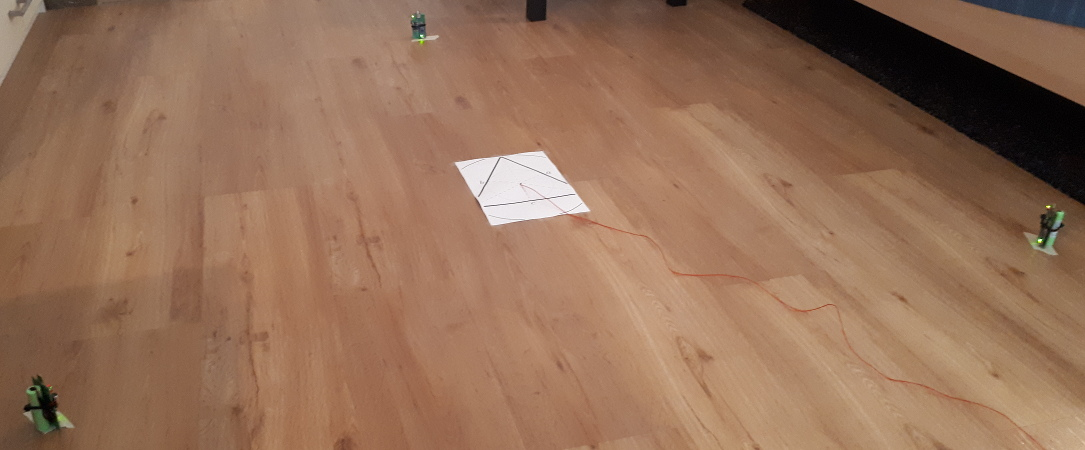
\includegraphics[width=0.9\linewidth]{calibration_triangle2}
	\caption{Versuchsaufbau für die Kalibierung von drei \Glsuseri{uwbm}.}
	\label{fig:calibration_triangle2}
\end{figure}

\begin{equation}
r_u = \frac{a}{3} \sqrt{3} \label{eq:dreieck_seitenlaenge_aus_umkreis}
\end{equation}

Initial wird die Antennenverzögerung bei allen \Glsuseri{uwbm} auf null gesetzt und danach reihum von jedem \Gls{uwbm} eintausend Entfernungsmessungen zu den beiden benachbarten \Glsuseri{uwbm} durchgeführt. Insgesamt entstehen dabei sechstausend Datensätze, die mittels dem \textit{LGS}-- bzw. des \textit{DecaWave}--Kalibrierungsverfahren ausgewertet werden, siehe \autoref{tab:calibration_antenna_delay_results}

Das \textit{LGS}--Kalibrierungsverfahren lieferte für jeden Durchlauf reproduzierbare Ergebnisse. Da jedes \Gls{uwbm} herstellungsbedingte Unterschiede aufweist, ist es Plausibel das alle Antennenverzögerungen in einem ähnlichen Wertebereich liegen. Anders sieht es bei dem \textit{DecaWave}--Kalibrierungsverfahren aus. Hier ergeben sich für jeden Durchlauf andere Wertekombinationen, bedingt durch die Zufallskomponente bei der Erstellung der Kandidatenliste. Diese Verhalten von Genetischen--Algorithmen ist bekannt und muss daher bei der Auswahl der Wertekombinationen berücksichtigt werden. Am Beispiel der Spalte \textit{DecaWave 1} wird es sehr deutlich. Hier beträgt der Unterschied zwischen dem größten und kleinsten Wert \approx\SI{23}{\ns} und entspricht damit einer Abweichung von \approx\SI{6}{\meter} zwischen diesen beiden \Glsuseri{uwbm}.

\begin{table}[h]
	\centering
	\begin{tabular}{||c||c||ccc||}
\hline
\Gls{uwbm} & LGS [\si{\second}] & DecaWave & DecaWave 1 & DecaWave 2 \\
\hline
\hline
176 & \num{257.45e9} & \num{242.48e9} & \num{232.21e9} & \num{254.50e9} \\
177 & \num{257.49e9} & \num{238.47e9} & \num{249.38e9} & \num{254.73e9} \\
178 & \num{257.11e9} & \num{257.17e9} & \num{255.36e9} & \num{215.07e9} \\
\hline
% Alte Darstellung
%176 & 16451 & 15494 & 14838 & 15912 & 16262 \\
%177 & 16453 & 15238 & 15935 & 15805 & 16277 \\
%178 & 16429 & 16433 & 16317 & 15131 & 13743 \\
	\end{tabular}
	\caption{Berechnete Werte für die Antennenverzögerung pro \Gls{uwbm}.}
	\label{tab:calibration_antenna_delay_results}
\end{table}

Die Wertekombinationen aus den Spalten \textit{LGS} und \textit{DecaWave} werden abwechselnd als Antennenverzögerungen in die \Glspl{uwbm} eingetragen und für jede Spalte jeweils eine weitere Messreihe, wie oben beschrieben, aufgezeichnet. Die Ergebnisse sind in der \autoref{tab:calibration_range_results} aufgeführt.

Mit einer initalen Antennenverzögerung von null beträgt die gemessene Entfernung zwischen zwei \Glsuseri{uwbm} \approx \SI{156}{\meter} bei einer tatsächenlichen Entfernung von \approx \SI{1.73}{\meter}. Eine Standardabweichung von \approx \SI{2}{\centi\meter} \footnote{Bei der Standardabweichung von über einem Meter handelt es sich um einen einzelnen Messfehler in der Messreihe.} entspricht dabei den Produkteigenschaften mit denen \textit{DecaWave} wirbt.

Werden die Antennenverzögerung aus der \textit{LGS}--Kalibrierungsverfahren benutzt, verbleibt die Standardabweichung in der gleichen Größenordnung wie im unkalibrierten Zustand. Jedoch nähert sich jetzt die gemessenen Entfernungen der tatsächlichen sehr stark an und bildet diesen sehr gut ab. Ganz im Gegensatz zu dem \textit{DecaWave}--Ka\-li\-brie\-rungs\-ver\-fa\-hren.

\begin{table}[h]
	\centering
	\begin{tabular}{||c||cc||ccc|cc||}
\hline
Kalibrierung & Tag & Anker & Entfernung [\si{\meter}] & $\overline{x}$ & $\sigma$ & Min & Max \\
\hline
\hline
Keine & 176 & 177 & \num{1.732} & \num{156.108} & \num{0.018} & \num{156.050} & \num{156.170} \\
Keine & 176 & 178 & \num{1.732} & \num{155.929} & \num{0.021} & \num{155.870} & \num{156.000} \\
Keine & 177 & 176 & \num{1.732} & \num{156.106} & \num{1.025} & \num{156.020} & \num{188.470} \\
Keine & 177 & 178 & \num{1.732} & \num{156.016} & \num{0.023} & \num{155.930} & \num{156.090} \\
Keine & 178 & 176 & \num{1.732} & \num{156.067} & \num{0.022} & \num{156.010} & \num{156.130} \\
Keine & 178 & 177 & \num{1.732} & \num{155.997} & \num{0.019} & \num{155.930} & \num{156.060} \\
\hline
LGS & 176 & 177 & \num{1.732} & \num{1.695} & \num{0.019} & \num{1.640} & \num{1.750} \\
LGS & 176 & 178 & \num{1.732} & \num{1.795} & \num{0.022} & \num{1.740} & \num{1.880} \\
LGS & 177 & 176 & \num{1.732} & \num{1.656} & \num{0.017} & \num{1.590} & \num{1.700} \\
LGS & 177 & 178 & \num{1.732} & \num{1.751} & \num{0.023} & \num{1.670} & \num{1.810} \\
LGS & 178 & 176 & \num{1.732} & \num{1.773} & \num{0.026} & \num{1.700} & \num{1.850} \\
LGS & 178 & 177 & \num{1.732} & \num{1.712} & \num{0.020} & \num{1.660} & \num{1.780} \\
\hline
DecaWave & 176 & 177 & \num{1.732} & \num{11.883} & \num{0.020} & \num{11.820} & \num{11.950} \\
DecaWave & 176 & 178 & \num{1.732} & \num{6.261} & \num{0.021} & \num{6.200} & \num{6.340} \\
DecaWave & 177 & 176 & \num{1.732} & \num{11.857} & \num{0.015} & \num{11.810} & \num{11.900} \\
DecaWave & 177 & 178 & \num{1.732} & \num{7.406} & \num{0.023} & \num{7.340} & \num{7.480} \\
DecaWave & 178 & 176 & \num{1.732} & \num{6.182} & \num{0.025} & \num{6.100} & \num{6.270} \\
DecaWave & 178 & 177 & \num{1.732} & \num{7.458} & \num{0.019} & \num{7.390} & \num{7.520} \\
\hline
	\end{tabular}
	\caption{Stochastische Eigenschaften der \Glspl{uwbm} ohne und mit Antennenkalibrierung bei einem Abstand von \SI{1.73}{\meter}.}
	\label{tab:calibration_range_results}
\end{table}

In der \autoref{fig:calibration_histograms} wurden die gemessenen Entfernungen als Histogramm dargestellt. Gut zu erkennen ist die Normalverteilung der Messwerte um den Mittelwert.

\begin{figure}[h]
	\centering
	\begin{subfigure}[b]{0.32\linewidth}
		\centering
		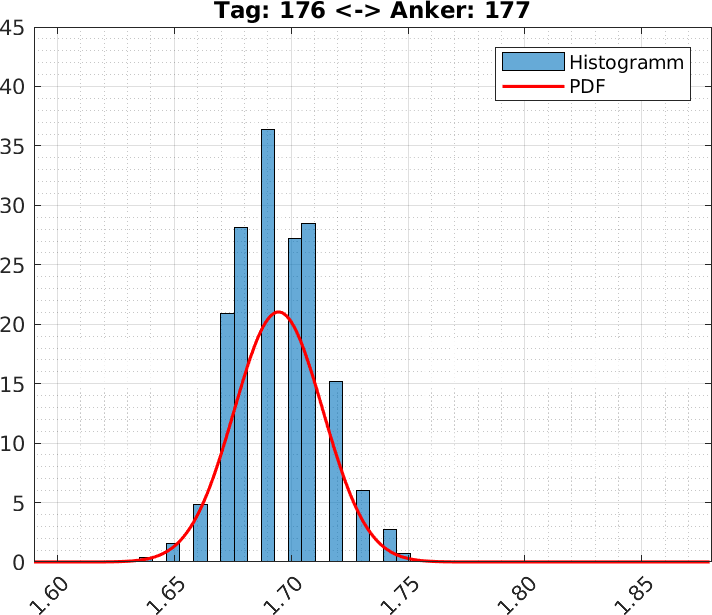
\includegraphics[width=\linewidth]{calibration_histogram_176_177}
	\end{subfigure}
	\hfill
	\begin{subfigure}[b]{0.32\linewidth}
		\centering
		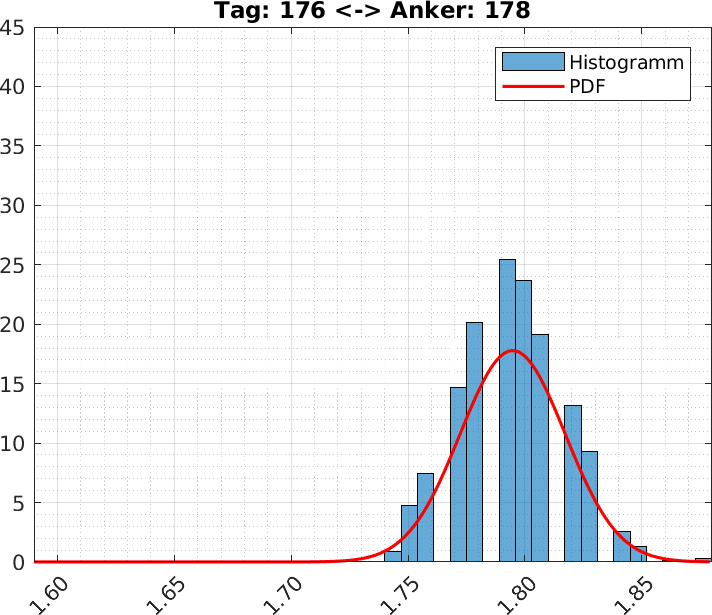
\includegraphics[width=\linewidth]{calibration_histogram_176_178}
	\end{subfigure}
	\hfill
	\begin{subfigure}[b]{0.32\linewidth}
		\centering
		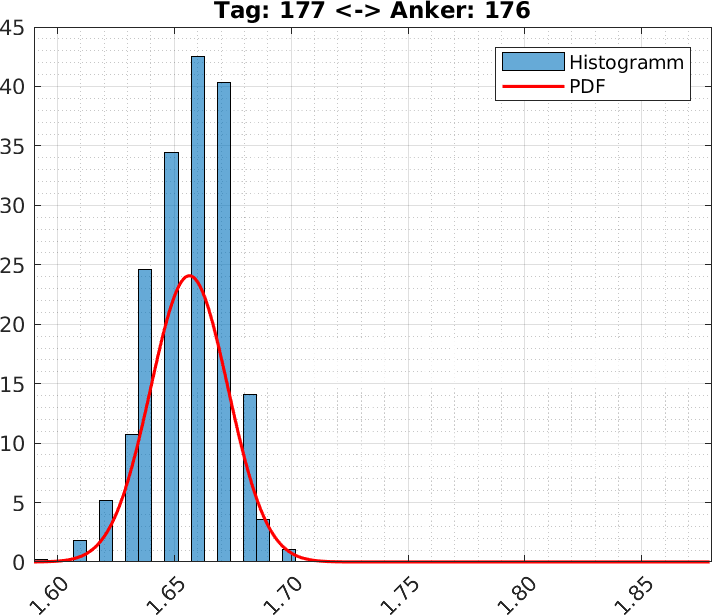
\includegraphics[width=\linewidth]{calibration_histogram_177_176}
	\end{subfigure}
	\par
	\bigskip
	\begin{subfigure}[b]{0.32\linewidth}
		\centering
		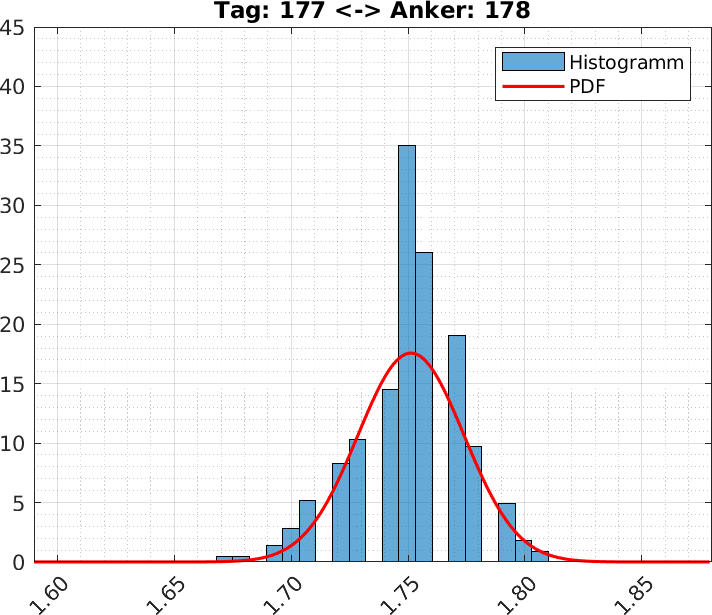
\includegraphics[width=\linewidth]{calibration_histogram_177_178}
	\end{subfigure}
	\hfill
	\begin{subfigure}[b]{0.32\linewidth}
		\centering
		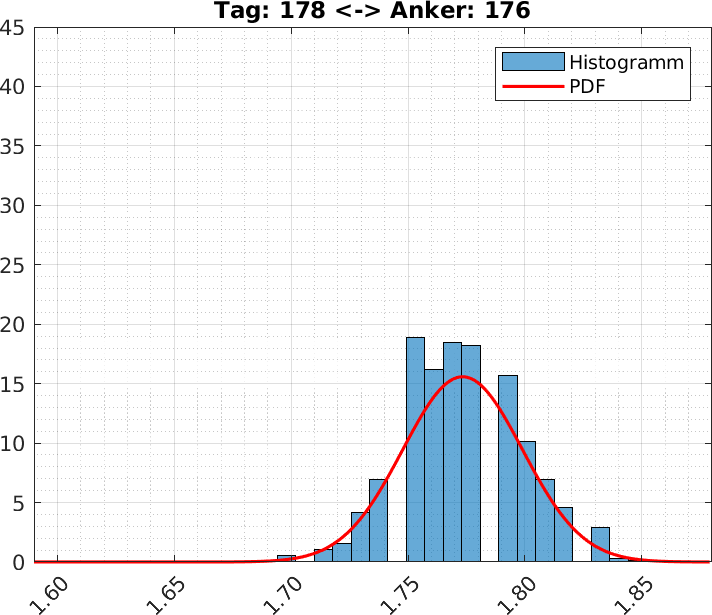
\includegraphics[width=\linewidth]{calibration_histogram_178_176}
	\end{subfigure}
	\hfill
	\begin{subfigure}[b]{0.32\linewidth}
		\centering
		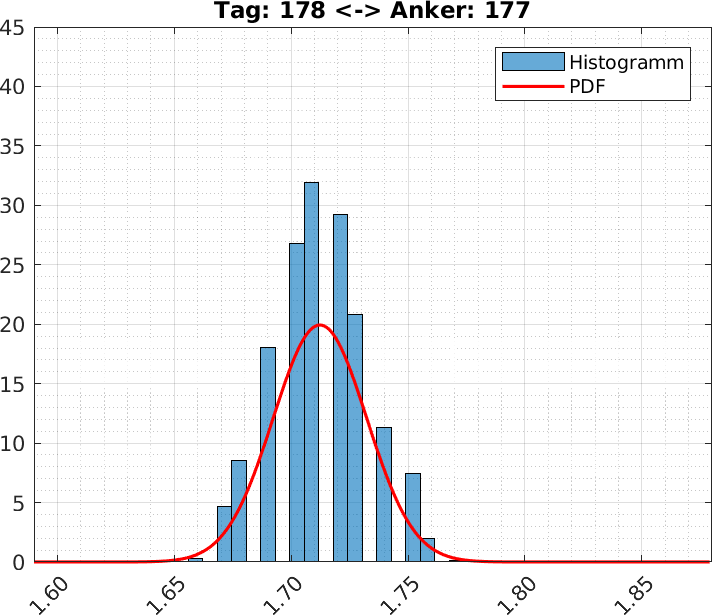
\includegraphics[width=\linewidth]{calibration_histogram_178_177}
	\end{subfigure}
	\caption{Histogramm und Wahrscheinlichkeitsdichtefunktion der kalibrierten Entfernungsmessungen.}
	\label{fig:calibration_histograms}
\end{figure}

Im zweiten Kalibriervorgang werden alle fünf \Glspl{uwbm} eingeschlossen. Jetzt reicht ein Dreieck nicht mehr aus, statt dessen wird ein Pentagramm verwendet, siehe \autoref{fig:calibration_pentagram2}. Dieses lässt sich mathematisch ähnlich gut beschreiben wie das Dreieck. Aus der Seitenlänge $a = \SI{4.5}{\meter}$, zwischen zwei benachbarten Spitzen, wird über die \autoref{eq:pentagramm_diagonale} der Abstand $d$, zwischen den diagonalen Spitzen, berechnet. Der Umkreisradius $r_u$ ergibt sich aus der \autoref{eq:pentagramm_umkreisradius}.

\begin{equation}
d = \frac{a}{2} \left(1 + \sqrt{5} \right) \label{eq:pentagramm_diagonale}
\end{equation}

\begin{equation}
r_u = \frac{a}{10} \sqrt{50 + 10 \sqrt{5}} \label{eq:pentagramm_umkreisradius}
\end{equation}

\begin{figure}[h]
	\centering
	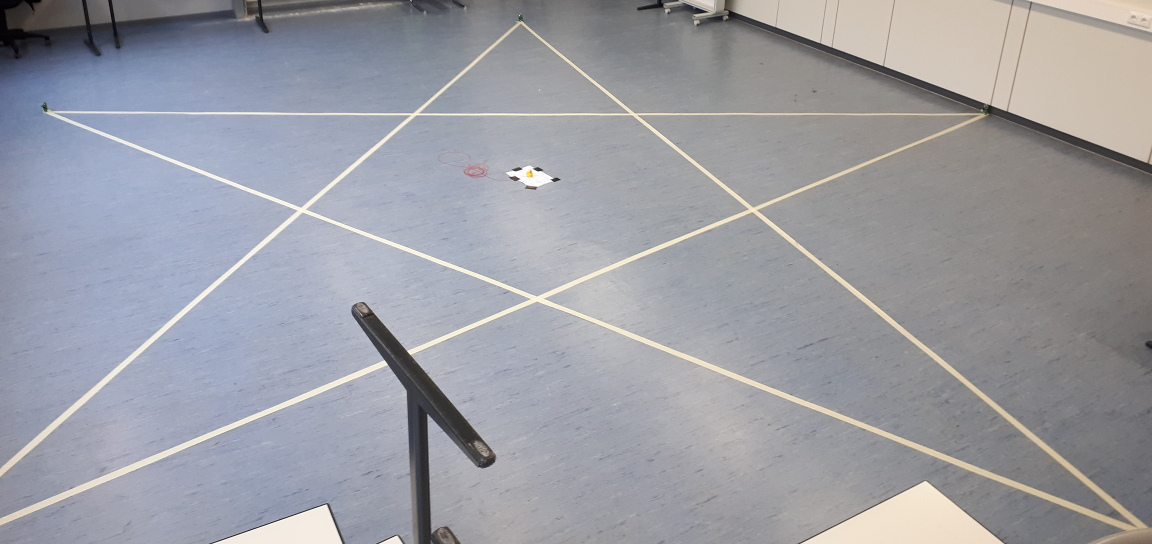
\includegraphics[width=0.9\linewidth]{calibration_pentagram2}
	\caption{Versuchsaufbau für die Kalibierung von fünf \Glsuseri{uwbm}.}
	\label{fig:calibration_pentagram2}
\end{figure}

Für das Pentagramm wurde nur noch das \textit{LGS}--Kalibrierungsverfahren verwendet, die Antennenverzögerungen pro \Gls{uwbm} sind dabei in der \autoref{tab:calibration_pentagramm_antenna_delay_results} aufgeführt.

\begin{table}[h]
	\centering
	\begin{tabular}{||c||c||}
\hline
\Gls{uwbm} & LGS [\si{\second}] \\
\hline\hline
176 & \num{257.30e9} \\
177 & \num{256.67e9} \\
178 & \num{256.67e9} \\
179 & \num{256.41e9} \\
180 & \num{257.20e9} \\

% Alte Darstellung
%176 & 16441 \\
%177 & 16401 \\
%178 & 16401 \\
%179 & 16384 \\
%180 & 16435 \\
\hline
	\end{tabular}
	\caption{Berechnete Werte für die Antennenverzögerung pro \Gls{uwbm} für das Pentagramm.}
	\label{tab:calibration_pentagramm_antenna_delay_results}
\end{table}


\begin{comment}
--------------------------------------------------------------------------------
- Wie verändert sich die Genauigkeit der Entfernungsmessung bei einer direkten Sichtverbindung (engl. Line--of--sight (LOS)) und indirekten Sichtverbindung (engl. Non--line--of--sight (NLOS))?
\end{comment}
\section{Entfernungsmessung [new]}

Um die Charakteristik der Entfernungsmessung zu bestimmen, wird eine \Gls{los}-- und drei \Gls{nlos}--Messreihen aufgezeichnet. Jede Messreihe beginnt bei einer Entfernung von einem Meter zwischen \Gls{tag} und \Gls{anchor}. Pro Entfernung werden jeweils fünfhundert Messwerte aufgezeichnet. Danach wird die Entfernung um einen halben Meter erhöht, indem der \Gls{anchor} verschoben wird. Dies erfolgt solange bis eine Entfernung von neun Meter erreicht ist. Somit enthält jede Messreihe siebzehn Entfernungen mit achttausendfünfhundert Entfernungsmessungen.

Bei der ersten \Gls{nlos}--Messreihe wird ein \SI{19x12x10}{\centi\meter} großer, mit Wasser gefüllter Kunststoffbehälter in einem Abstand von \SI{2}{\centi\meter} vor der \Gls{uwb}--Antenne platziert, siehe \autoref{fig:entfernungsmessung_versuchsaufbau_20180120_133013}. Bei den letzten zwei \Gls{nlos}--Messreihen wird ein \SI{44x25}{\centi\meter} großes Aluminiumblech mit einer Dicke von \SI{0.5}{\milli\meter} vor die \Gls{uwb}--Antenne platziert, jeweils in einem Abstand von \SI{5}{\centi\meter} und \SI{50}{\centi\meter}, siehe \autoref{fig:entfernungsmessung_versuchsaufbau_20180120_122434} und \autoref{fig:entfernungsmessung_versuchsaufbau_20180120_140118}.

\begin{figure}[ht]
	\begin{minipage}{0.49\linewidth}
		\begin{subfigure}{\linewidth}
			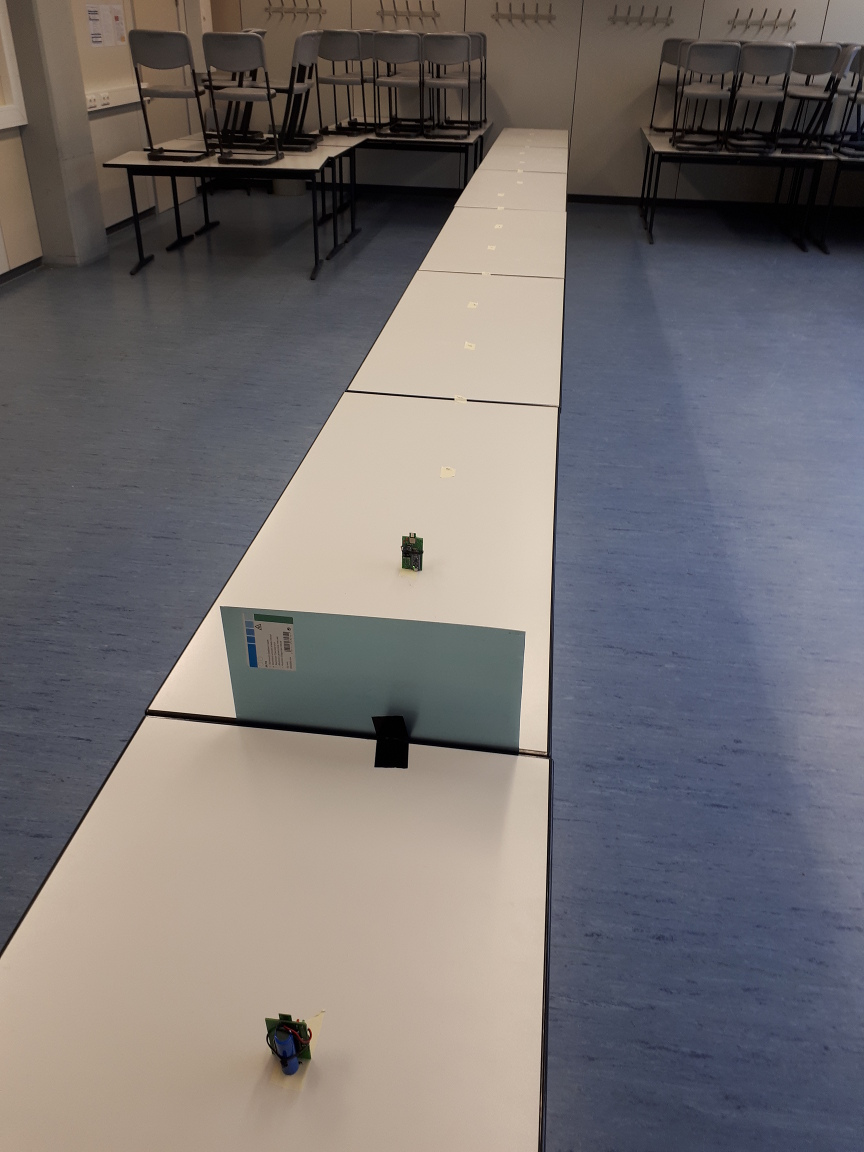
\includegraphics[width=\linewidth]{entfernungsmessung_versuchsaufbau_20180120_122434_2}
			\caption{ }
			\label{fig:entfernungsmessung_versuchsaufbau_20180120_122434}
		\end{subfigure}
	\end{minipage}
	\hfill
	\begin{minipage}{0.49\linewidth}
			\begin{minipage}{\linewidth}
				\begin{subfigure}{\linewidth}
					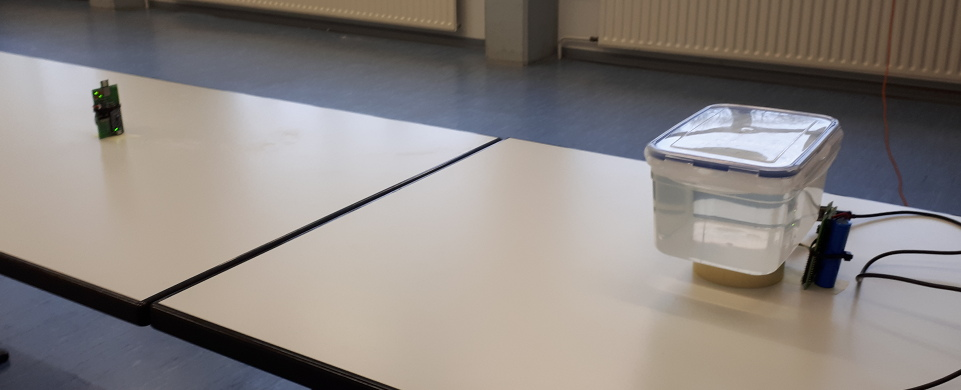
\includegraphics[width=\linewidth]{entfernungsmessung_versuchsaufbau_20180120_133013_2}
					\caption{ }
					\label{fig:entfernungsmessung_versuchsaufbau_20180120_133013}
				\end{subfigure}
			\end{minipage}
			\par
			\bigskip
			\begin{minipage}{\linewidth}
				\begin{subfigure}{\linewidth}
					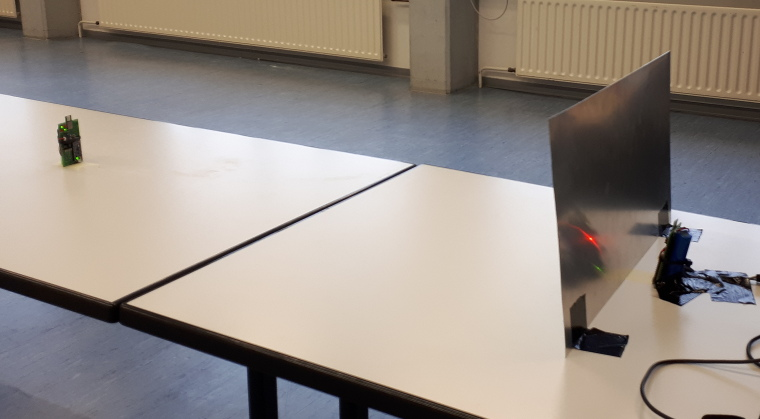
\includegraphics[width=\linewidth]{entfernungsmessung_versuchsaufbau_20180120_140118_2}
					\caption{ }
					\label{fig:entfernungsmessung_versuchsaufbau_20180120_140118}
				\end{subfigure}	
			\end{minipage}
	\end{minipage}
	\caption{Versuchsaufbau für die \Gls{nlos}--Entfernungsmessung.}
	\label{fig:entfernungsmessung_versuchsaufbau_20180120}
\end{figure}


Das auffälligste Merkmal der \Gls{los}-- als auch der \Gls{nlos}--Entfernungsmessungen ist die systematische Verschiebung aller Messwerte um ca. \SI{20}{\centi\meter} deren Ursache ungeklärt bleibt, siehe \autoref{fig:entfernungsmessung_2018_01_20}.

Bei der \Gls{los}--Messreihe beträgt die Standardabweichung, wie bereits bei der Kalibrierung, ca. \SI{2}{\centi\meter}. Mit steigender Entfernung steigt auch die Standardabweichung von ca. \SI{1.8}{\centi\meter} bei einem Meter auf ca. \SI{2.3}{\centi\meter} bei neun Meter an. Größere Ausreißer sind bei den Messwerten nicht vorhanden, siehe \autoref{fig:entfernungsmessung_2018_01_20_los} und \autoref{tab:entfernungsmessung_2018_01_20_los}.

In der \autoref{fig:entfernungsmessung_2018_01_20_nlos_water} ist deutlich zu erkennen, das Wasser einen sehr störenden Einfluss auf die Entfernungsmessung ausübt. Die Messwerte streuen über einen sehr großen Bereich, das spiegelt sich auch in der Standardabweichung, die im besten Fall ca. \SI{5}{\centi\meter} und im schlimmsten Fall ca. \SI{34}{\centi\meter} beträgt, siehe \autoref{tab:entfernungsmessung_2018_01_20_nlos_water}.

Ähnlich verhält es sich bei der \Gls{nlos}--Messreihe mit einem Aluminiumblech, das sehr nah vor der \Gls{uwb}--Antenne platziert wurde, siehe \autoref{fig:entfernungsmessung_2018_01_20_nlos_metal2} und \autoref{tab:entfernungsmessung_2018_01_20_nlos_metal2}. Einzig im Bereich von zwei bis fünf Meter beträgt die Standardabweichung ca. \SI{2}{\centi\meter}.

Keinen besonders großen Einfluss hat das Aluminiumblech, wenn es sich in einer Entfernung von \SI{50}{\centi\meter} befindet. Die Werte der Standardabweichung ähneln der \Gls{los}--Messreihe. Nur im Bereich zwischen achteinhalb und neun Meter steigt die Standardabweichung auf einen Wert von ca. \SI{30}{\centi\meter} an. Dies könnte darauf zurückzuführen sein, das im hinteren Bereich des Raums Metallstühle auf den Tischen standen, siehe \autoref{fig:entfernungsmessung_versuchsaufbau_20180120_122434}.


\begin{figure}[ht]
	\centering
	\begin{subfigure}[t]{0.49\linewidth}
		\centering
		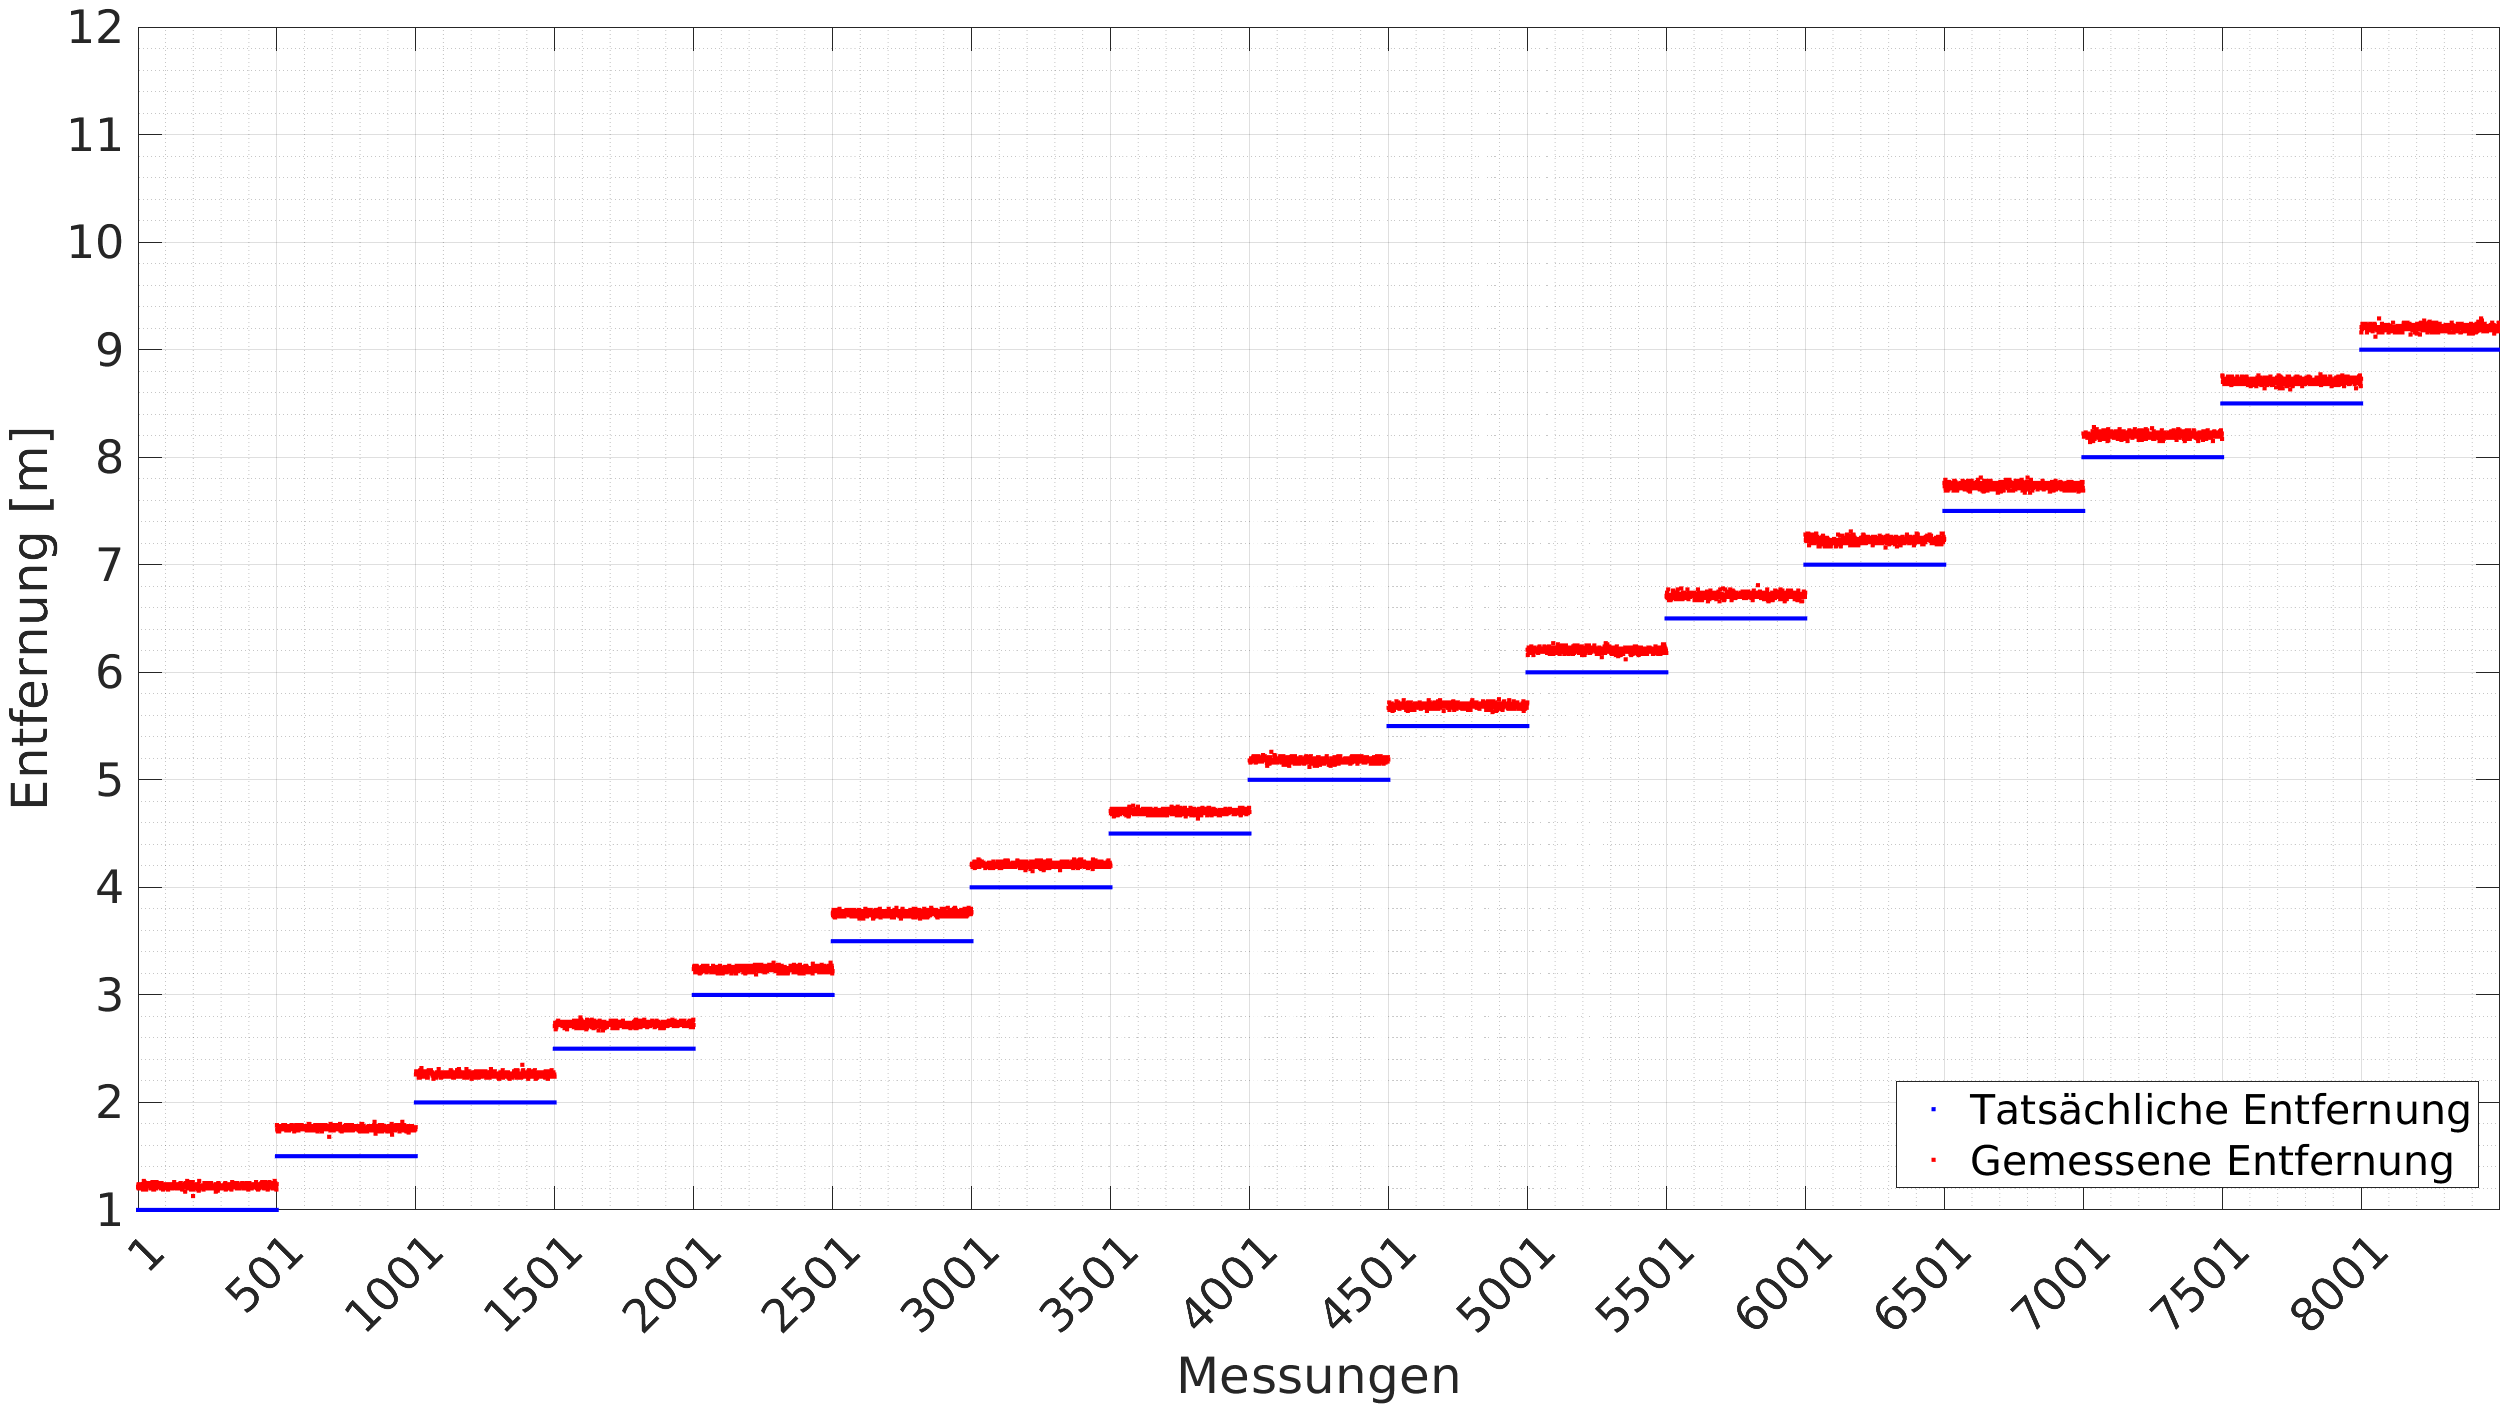
\includegraphics[width=\linewidth]{entfernungsmessung_2018_01_20_los}
		\caption{\Gls{los}}
		\label{fig:entfernungsmessung_2018_01_20_los}
	\end{subfigure}
	\hfill
	\begin{subfigure}[b]{0.49\linewidth}
		\centering
		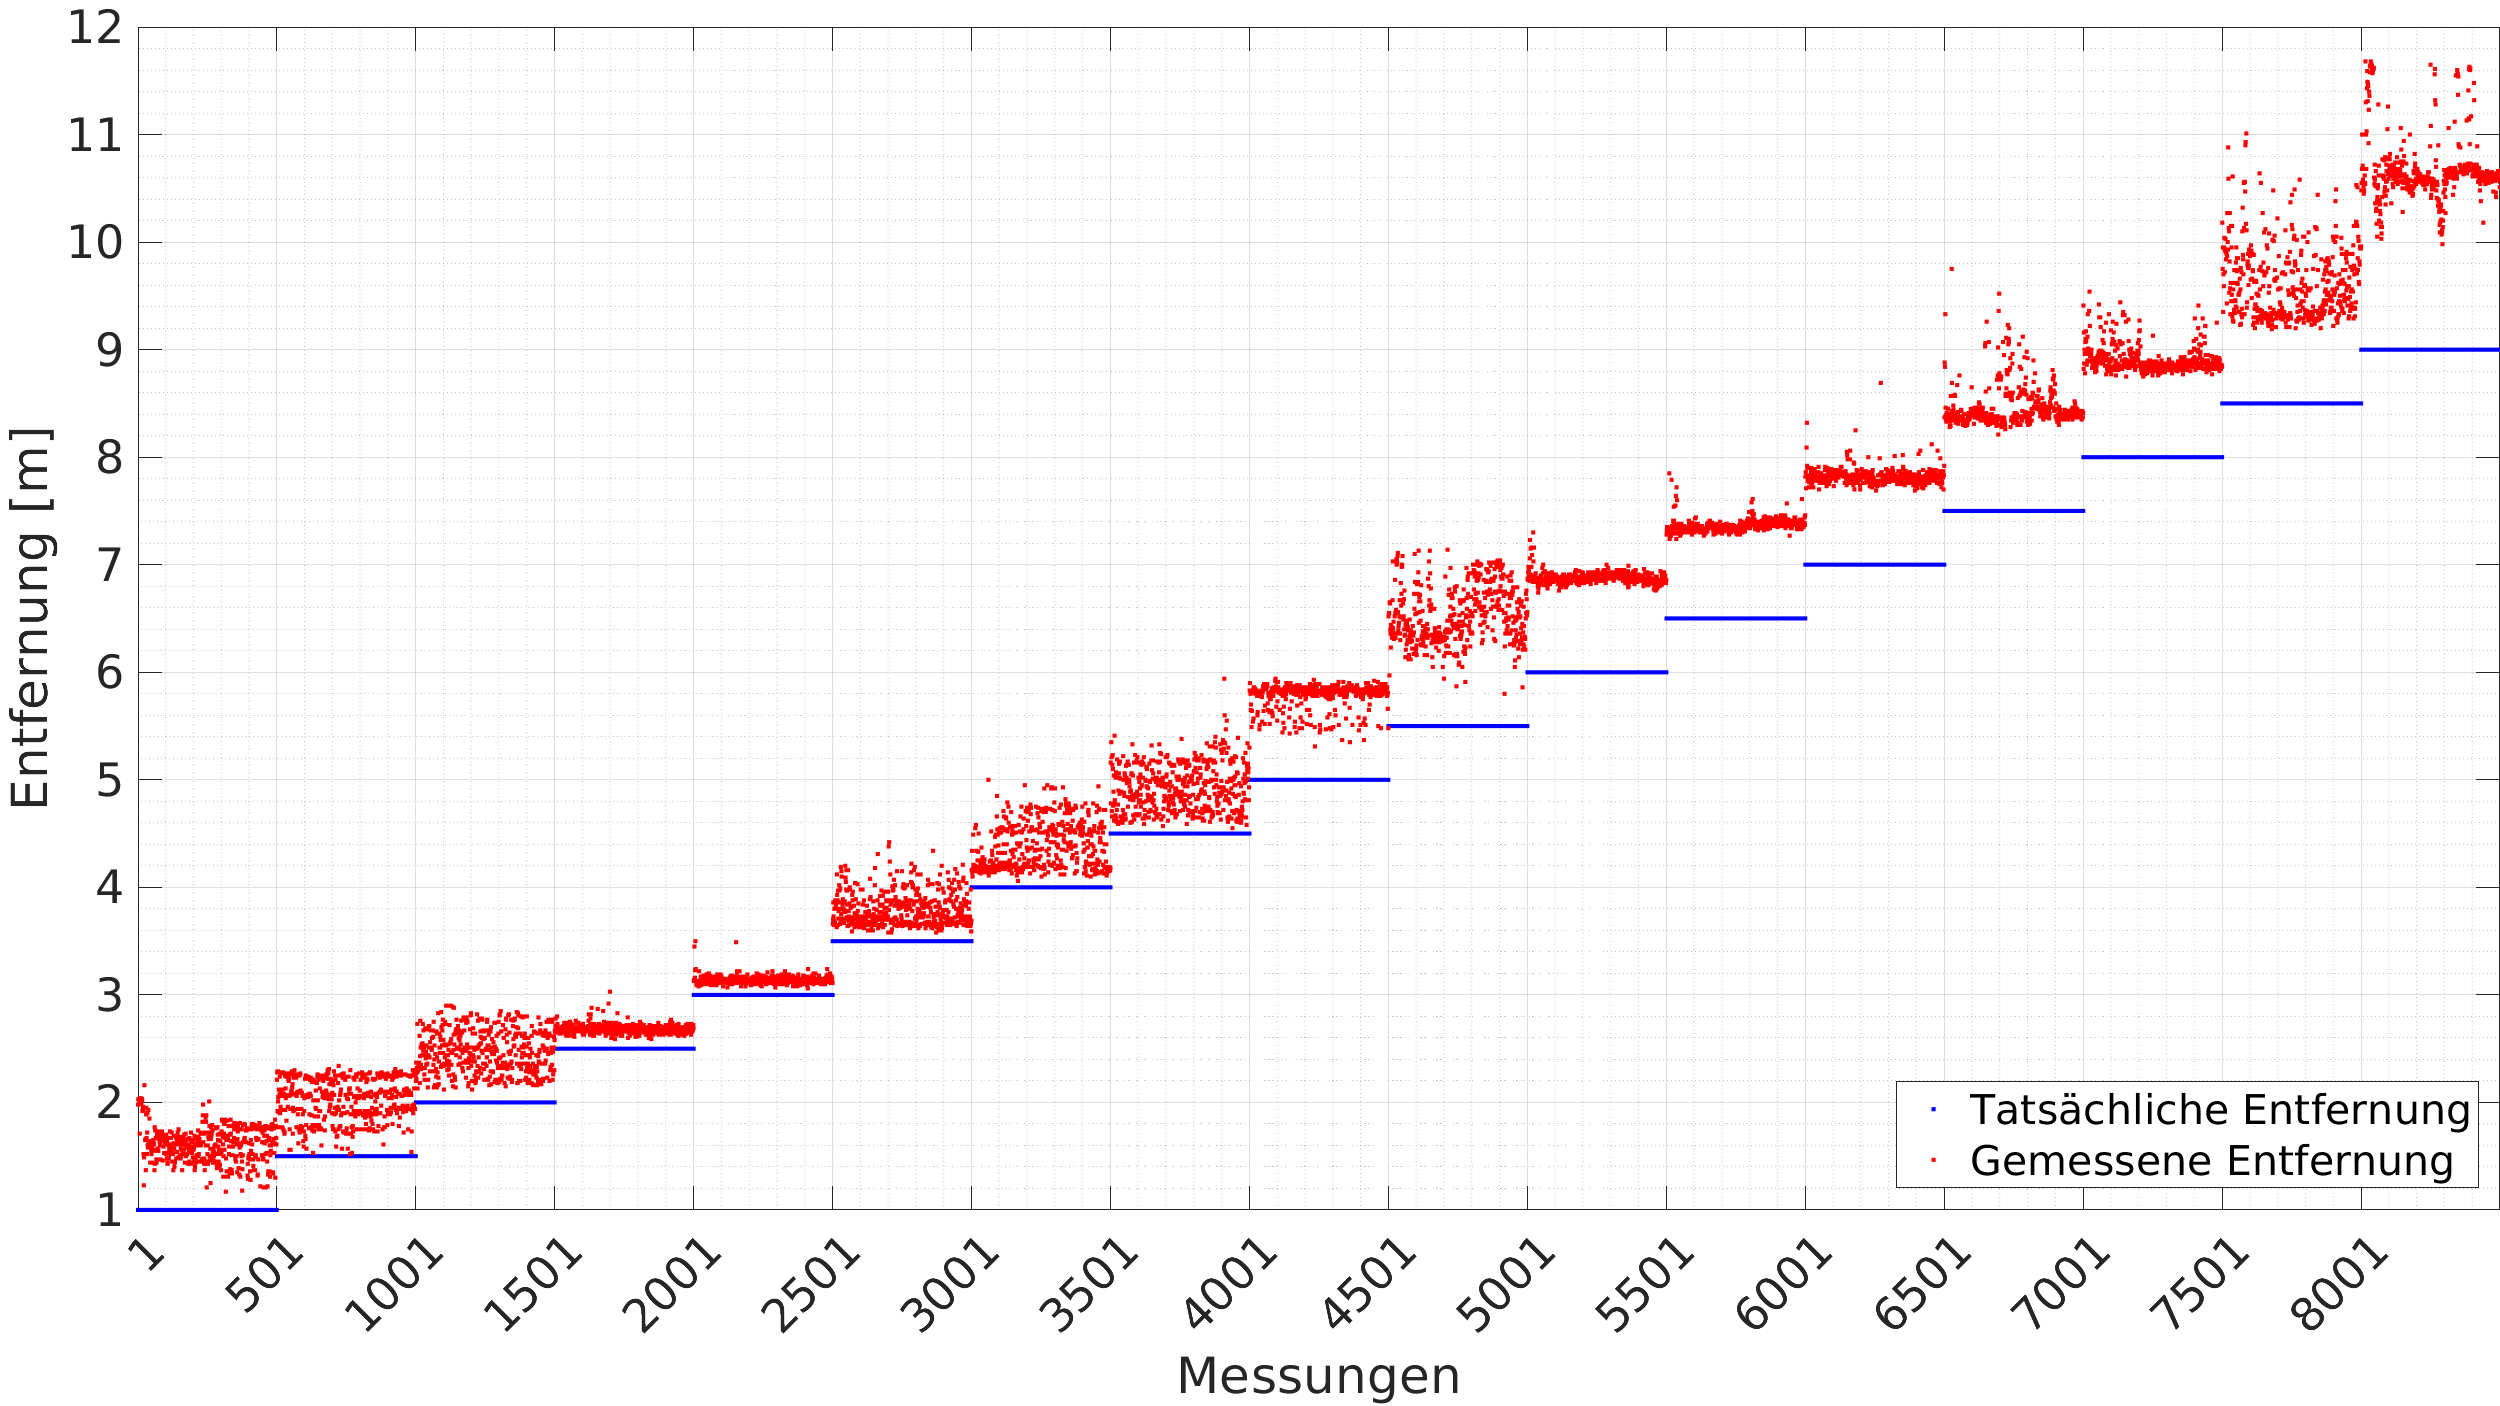
\includegraphics[width=\linewidth]{entfernungsmessung_2018_01_20_nlos_water}
		\caption{\Gls{nlos} mit einem wassergefüllten Kunststoffbehälter.}
		\label{fig:entfernungsmessung_2018_01_20_nlos_water}
	\end{subfigure}
	\par
	\bigskip
	\begin{subfigure}[b]{0.49\linewidth}
		\centering
		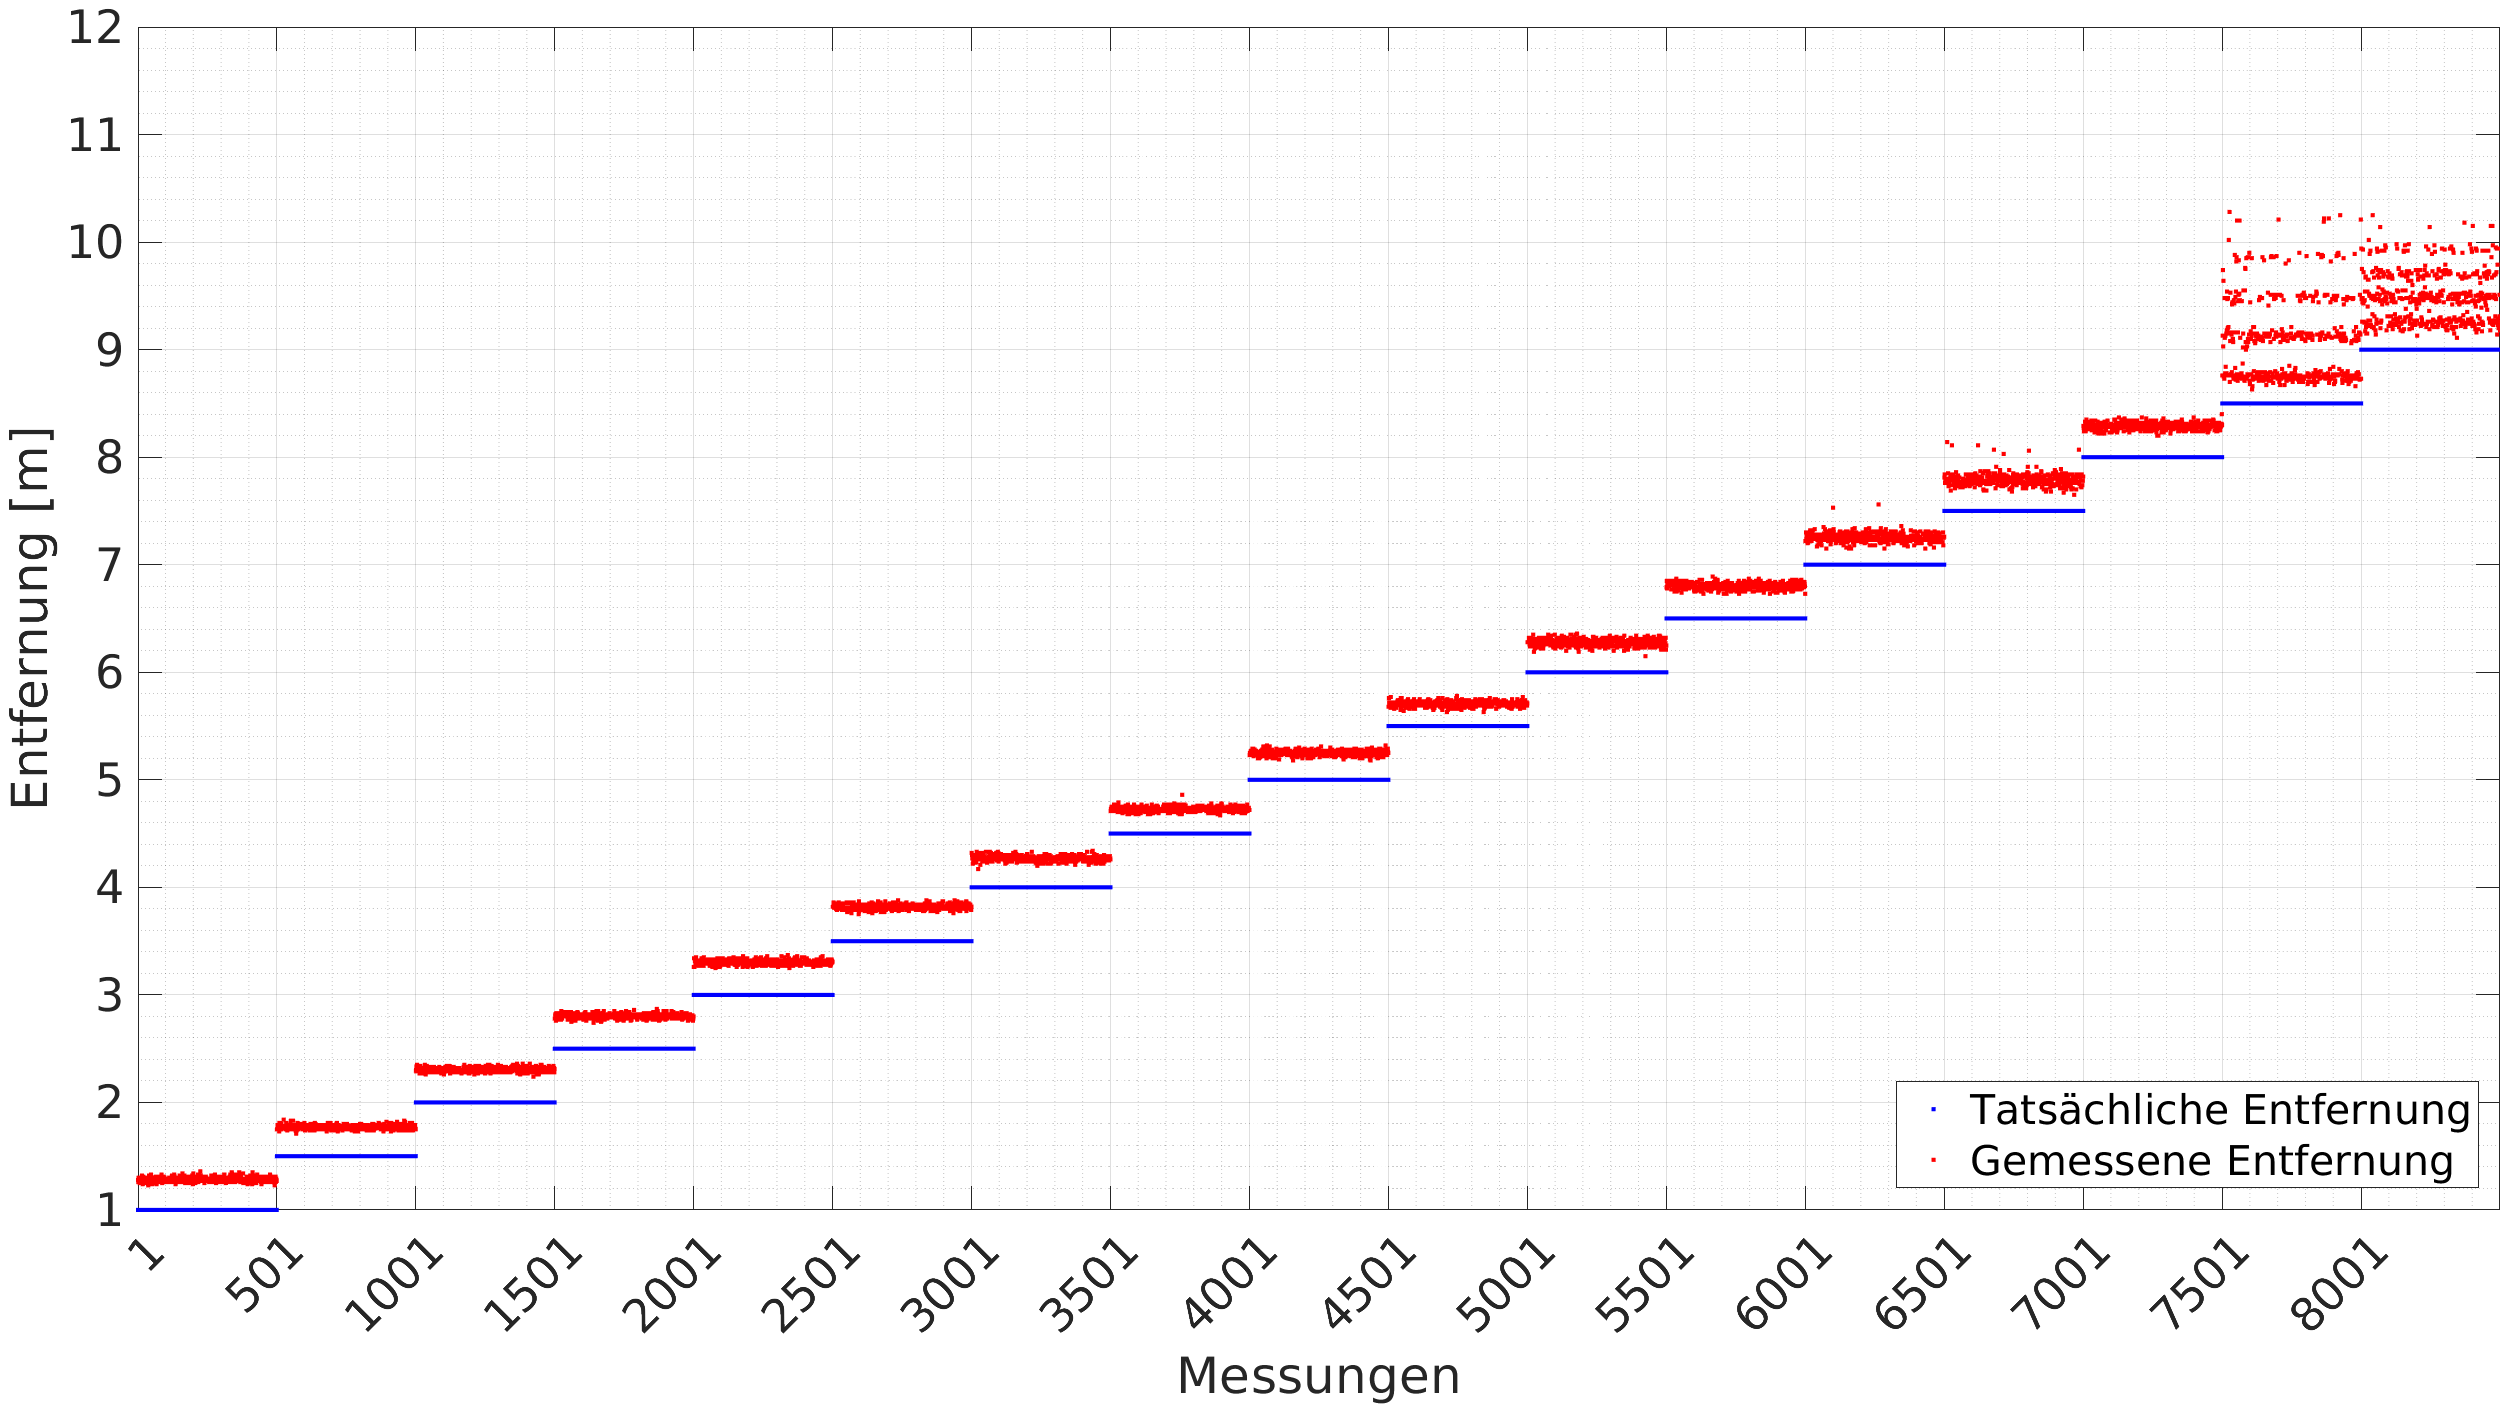
\includegraphics[width=\linewidth]{entfernungsmessung_2018_01_20_nlos_metal}
		\caption{\Gls{nlos} mit einem Aluminiumblech in einer Entfernung von \SI{50}{\centi\meter}.}
		\label{fig:entfernungsmessung_2018_01_20_nlos_metal}
	\end{subfigure}
	\hfill
	\begin{subfigure}[b]{0.49\linewidth}
		\centering
		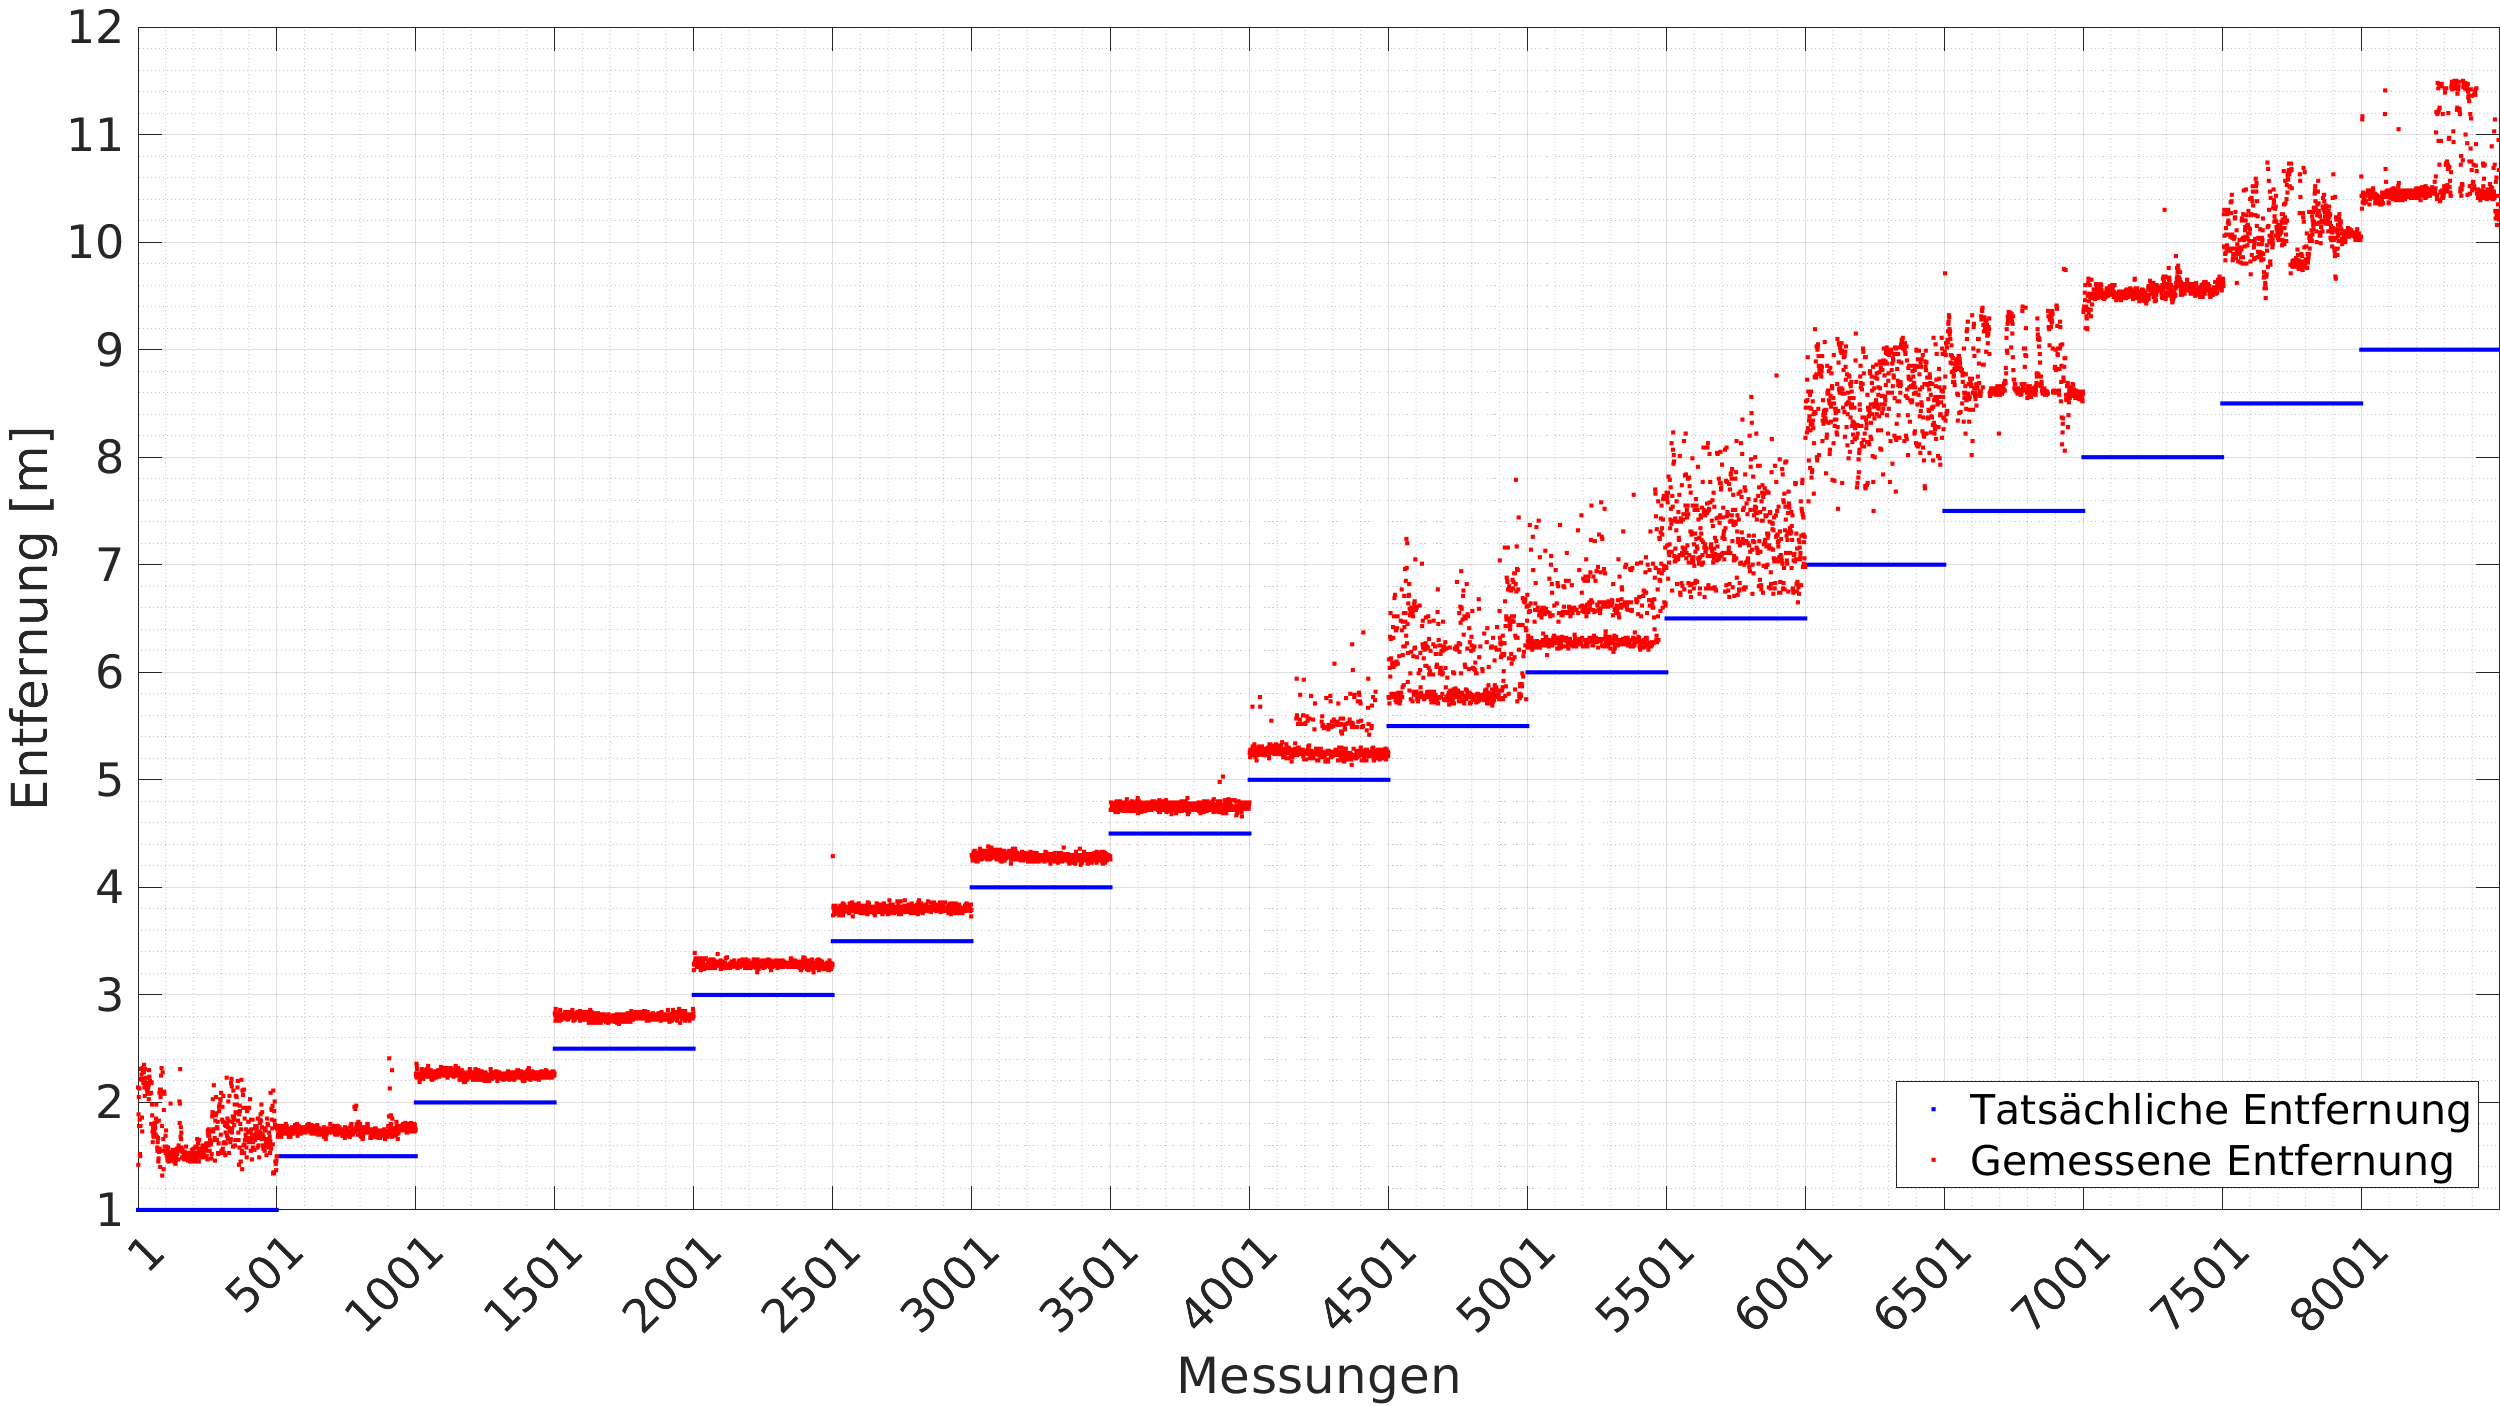
\includegraphics[width=\linewidth]{entfernungsmessung_2018_01_20_nlos_metal2}
		\caption{\Gls{nlos} mit einem Aluminiumblech in einer Entfernung von \SI{5}{\centi\meter}.}
		\label{fig:entfernungsmessung_2018_01_20_nlos_metal2}
	\end{subfigure}
	\caption{Tatsächliche und gemessene \Gls{los}--und \Gls{nlos}--Entfernungen.}
	\label{fig:entfernungsmessung_2018_01_20}
\end{figure}


\begin{comment}
--------------------------------------------------------------------------------
- Diagramme
	- \cite{kurth2003experimental}
		- Fig. 5: (1) The ground truth path with tags indicated by circles. The numbers indicate how many range measurements were received from each tag over the duration of Test 1. (2) The path estimate from dead reckoning alone. (3) The path estimate from localization using a Kalman Filter. The Filter fuses data from odometry and a gyro with absolute measurements from RF tags to produce this path estimate. Numerical results are given in Table 1. (X: position in x(m), Y: position in y(m), Ground truth path with tag locations, Dead reckoning path, Kalman filter localization path)

		
- Versuchsbeschreibung:
	- Warum wurden die uwbm da platziert wo sie jetzt stehen?
	
\end{comment}
\section{RO-SLAM [todo]}


\begin{comment}
--------------------------------------------------------------------------------
\end{comment}
\subsection{Trajektorie [todo]}


\begin{comment}
--------------------------------------------------------------------------------
\end{comment}
\subsection{Vergleich von MC und SOG [todo]}

